\begin{figure*}
    \centering
    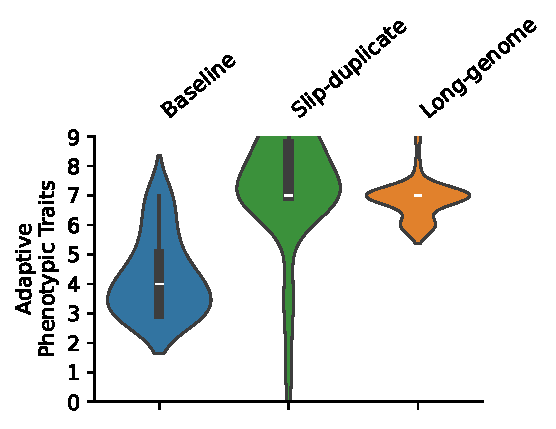
\includegraphics[width=0.5\linewidth]{binder/binder/teeplots/adaptive-evolution-rate.ipynb/hue=treatment+inner=box+kind=violin+mutation=per site+viz=catplot+x=treatment+y=has-task+ext=.pdf}%
    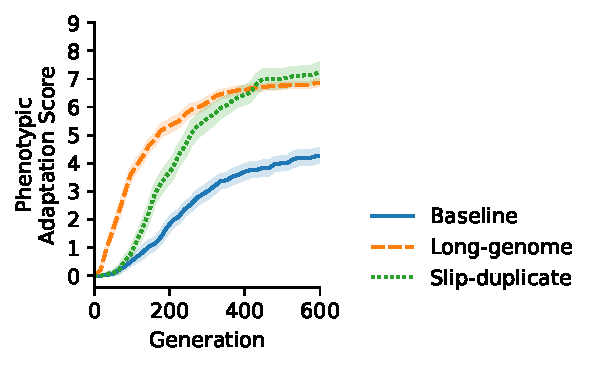
\includegraphics[width=0.5\linewidth]{binder/binder/teeplots/adaptive-evolution-rate.ipynb/errorbar=se+hue=treatment+kind=line+mutation=per site+style=treatment+viz=relplot+x=generation+y=has-task+ext=.pdf}
    \caption{
        \textbf{Aggregated adaptive evolution of phenotypic traits for long-genome control experiments.}
        \small Violin plots show number of adaptive phenotypic traits evolved in final dominant genotypes.
        Time series (\ref{fig:results_panels:time_series} right) shows progression of adaptive phenotypic trait count along lineages of final dominant genotypes; color-coding corresponds to violin plots.
        Error bands give 95\% CI, bootstrapped over 30 replicates per treatment.
    }
    \label{fig:adaptive-evolution-rate-agg}
\end{figure*}
